\section{\system: In-situ Analysis}\label{sec:system}
\system backend features an in-memory dataframe, a versioning database, a compiler for translating \vta commands that the execution engine runs, and a session manager to manage data, code, and visualizations. Figure~\ref{fig:arch} shows the overview of the \system system architecture. The components with dashed borders (``- -'') are partially implemented and require further refinement. We discuss the front-end components later.

\subsection{Data Model}
The underlying data structure of \system is a dataframe. A dataframe is a multidimensional array, $A_{mn}$, with a vector of row labels, $R = \{R_1, R_2, \ldots, R_m\}$ and a vector of column labels, $C = \{C_1,C_2,\ldots,C_n\}$~\cite{modin}. 
We opted for dataframes instead of a database since 
\vita tasks
(\eg featurization, classification) cannot always be conveniently performed inside the database~\cite{lajus2014efficient}.
Dataframes are widely used in
exploratory data analysis, including \vita due to their coverage of a wide variety of data analysis operators~\cite{modin}. 
%The \emph{Pandas} dataframe API within Python (pandas.pydata.org)
%has been downloaded more than 300 million times and served as a
%dependency for over 265,000 repositories in GitHub. 
They also do not require data to be defined schema-first allowing flexibility in supported data types and data structures. Finally, dataframes provide a functional interface suitable for REPL-style \vita workflows to perform ``quick and dirty'' analysis.

\begin{figure}[tbp] 
%\vspace{-20pt}
  \centering
  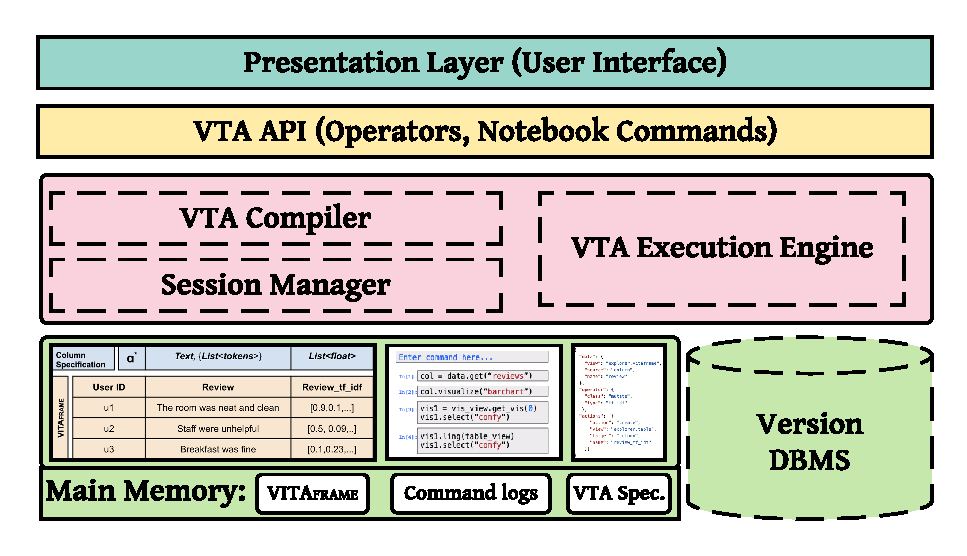
\includegraphics[width=\linewidth,trim={0 15 0 10},clip]{figures/vita.pdf}
  \caption{\small \system system architecture.\label{fig:arch}}
 \vspace{-15pt}
\end{figure}
To support \vita use-cases,  we assign a schema to dataframe columns---each column $C_i \in C$ may have a schema defined over a set of data domains, $D = \{d_1, d_2, \ldots\}$ that spans heterogeneous data types like text, visualizations (\textbf{D3}). We call this data structure a \vitaframe. We discuss the underlying data domain for \vita in Section~\ref{sec:vta}.
The REPL-style \vita workflows involve users creating and examining intermediate results that are also from the data domain, $D$. An intermediate result with one-to-one correspondence with a \vitaframe column
(\eg $n$ reviews are featurized into $n$ feature vectors) is added as a new column. However, these results may not have one-to-one correspondence (\eg dictionary of words in the set of $n$ reviews) and are stored in a separate data structure as metadata of the corresponding column.
Therefore, for each column $C_i \in C$ in a \vitaframe, there is a schema specification function that assigns a domain $d_j \in D$ to the column and a domain $d_k \in D$ for each column metadata (see Figure~\ref{fig:column_spec}).
%For example, in Figure~\ref{fig:column_spec}, the column \emph{Review}'s type is $Text$ and metadata type is $\mathbf{List}(\mathbf{token})$ (\ie the list of unique tokens in the text reviews). 
Metadata are often used for computing aggregate statistics and visualizations.
%For example, to visualize TF-IDF score of top ranked words in the reviews, a user can first construct a new metadata of type $\mathbf{Dictionary}(\mathbf{token}, \mathbf{float})$ that contains the average TF-IDF score of the unique tokens. Then they can use the metadata to create and visualize a ranked list of words as a bar chart (see Figure~\ref{fig:use-case-a}c).
% Note that there can be columns with no metadata.}


\begin{figure}[!htb] 
\vspace{-10pt}
  \centering
  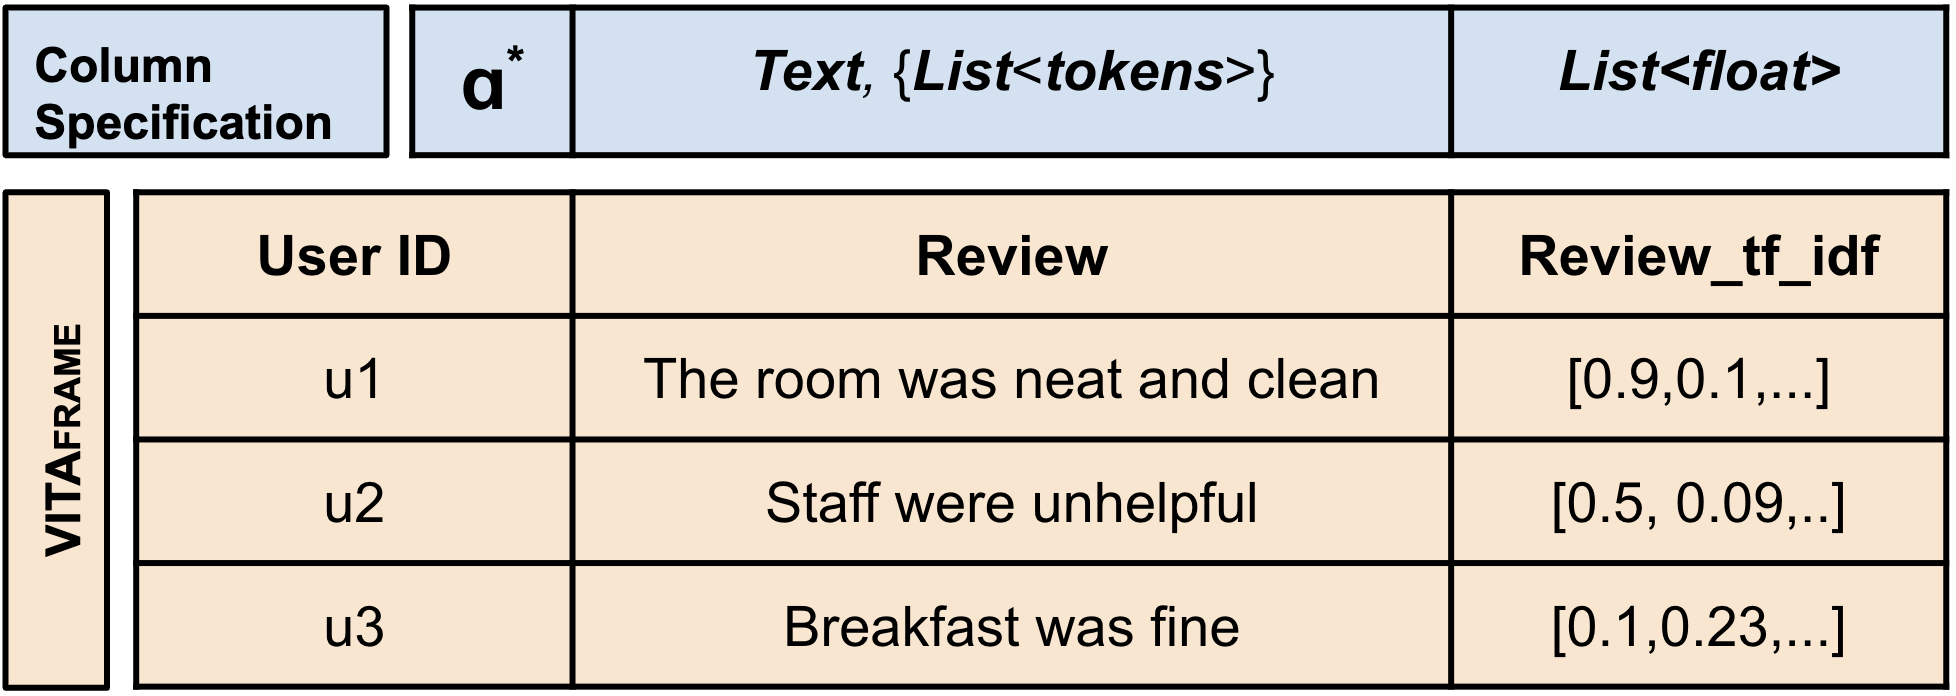
\includegraphics[width=\linewidth]{figures/column_spec.png}
  \caption{\small \vitaframe with column and metadata schema specification. The Review column is of type $\mathbf{Text}$ and the metadata, the collection of unique tokens, is of type $\mathbf{List}(\mathbf{token})$.\label{fig:column_spec}} 
  \vspace{-13pt}
\end{figure}

\subsection{Computation Model}\label{sec:computation}
\stitle{\vta Compiler.} 
In Section~\ref{sec:vta}, we present \vta,  an algebra for specifying \vita operations. \system compiles the user interactions on Operator View (see in Figure~\ref{fig:fe}a) or \vta commands in Notebook View (see in Figure~\ref{fig:fe}d) into \vta specifications. However, the \vta specifications are incomplete, in the sense that they may omit details ranging from visual encoding such as fonts, line widths to input data type.
To resolve these ambiguities \system currently uses a rule-based compiler that translates 
a \vta specification into lower-level operators for the execution engine to run backend computation (see Section~\ref{sec:vta}).

\begin{figure*}
\centering
\small
\begin{tabular}{ c c c}
  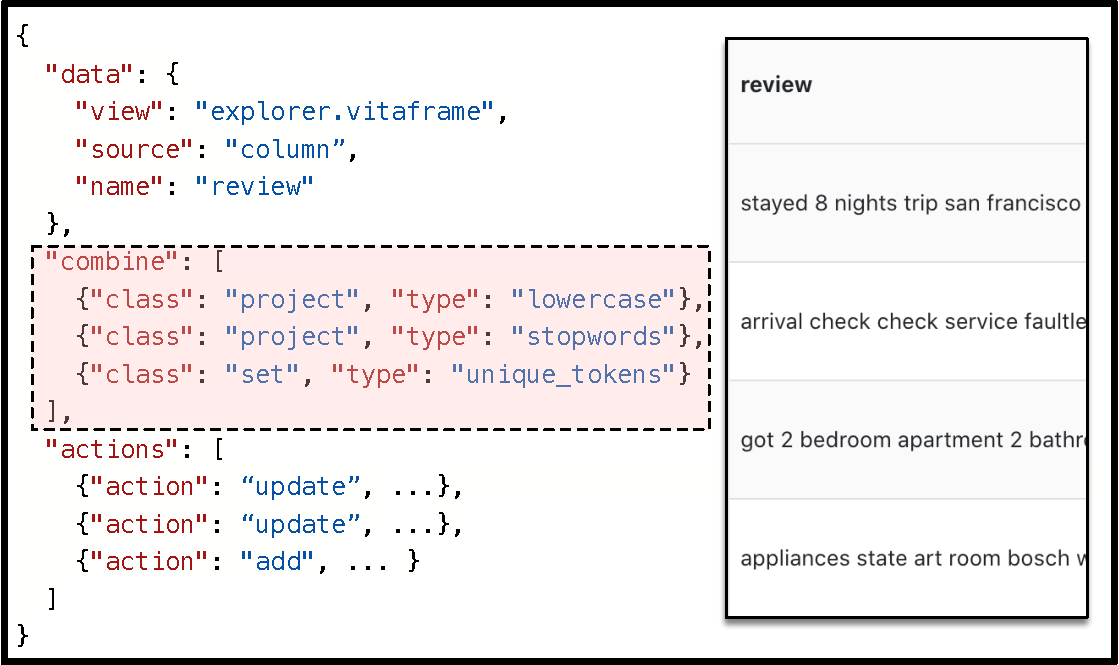
\includegraphics[width=0.3\linewidth,height=0.18\linewidth]{figures/combine_clean.pdf}   & 
  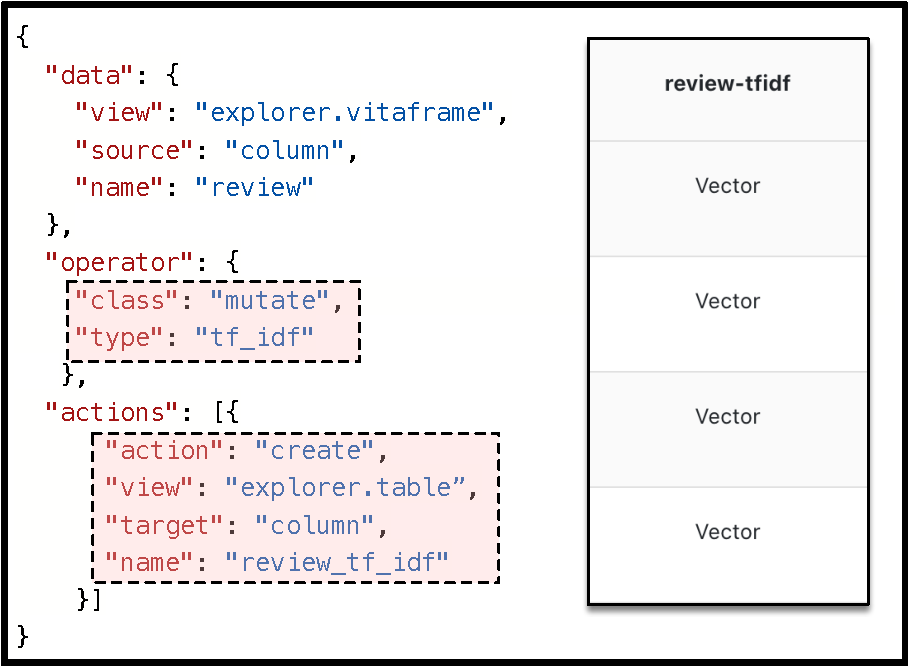
\includegraphics[width=0.3\linewidth,height=0.18\linewidth]{figures/tf_idf.pdf} & 
  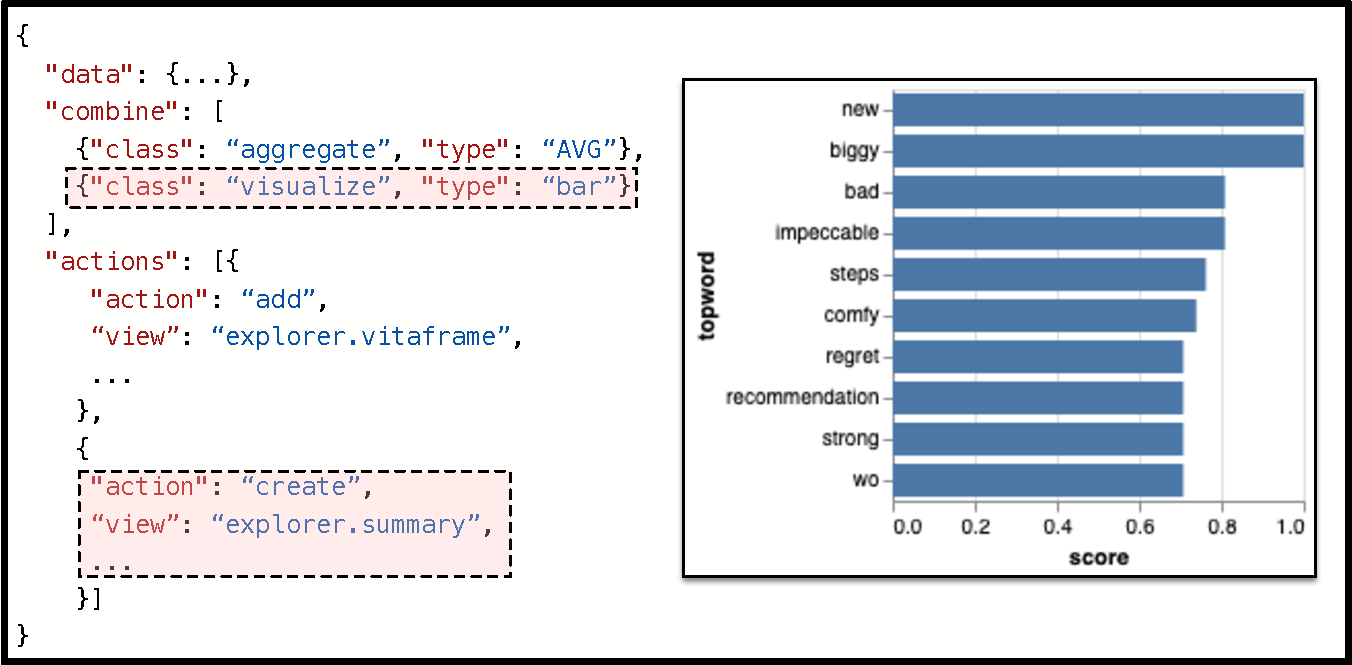
\includegraphics[width=0.4\linewidth,height=0.18\linewidth]{figures/barchart.pdf} \\
     (a) Clean and generate metadata & 
     (b) Create TF-IDF feature vector &
     (c) Visualize top-words by TF-IDF score
\end{tabular}
    \caption{\small \vta specification. (a) Create a composite cleaning operator ( \code{lowercase} and \code{remove\_stopwords}) using \code{combine} and generate metadata (\code{unique\_tokens}). (b) Create TF-IDF vectors from reviews using \code{mutate} operator (added as a new column in Table View). (c) Create a bar chart by combining \code{aggregate} (average TF-IDF score for each token) and \code{visualize} operator.}
\vspace{-15pt}
    \label{fig:use-case-a}
\end{figure*}

\stitle{Execution Engine.} 
The \vita execution engine takes the following input generated by the \vta compiler: (1) input data schema in $D$ 
and (2) translated \vta specifications. The text analysis operations---data preprocessing,
featurization, 
feature transformation/selection),
estimation),
and more advanced post-processing operations
like anomaly detection---are mapped to existing ML and NLP libraries like Spacy, Scikit-learn. While other \vta operators related to visual coordination are mapped to built-in implementations (see Section~\ref{sec:vta}).

% \candidate{The text analysis operations---data preprocessing (\eg cleaning),
% feature extraction (\eg TF-IDF featurization), 
% feature transformation/selection (\eg PCA),
% estimation (\eg classify),
% and more advanced post-processing operations
% (\eg anomaly detection)---are mapped to existing ML and NLP libraries like Spacy, Scikit-learn. While other \vta operators related to visual coordination are mapped to built-in implementations.}

\stitle{Version Control.}
After each operation, \system checkpoints the current state of the visualizations, \vitaframe, and notebook commands. The development of a fully functional system for fine-grained (\ie at operation level) versioning is currently in progress (\textbf{D5}). 
 We discuss how to support fine-grained version management of a \vita session involving heterogeneous data types, notebook commands, and user interactions in
 Section~\ref{sec:discussion}.



\subsection{\system Front End}\label{sec:ui}
\system user interface has four components---Operator View, Table View, Visualization View, and Notebook View (see Figure~\ref{fig:fe})---which enables users to perform in-place text analytics (\textbf{D1}). Users can perform various \vita operations using the operators in Operator View (see Figure~\ref{fig:fe}a). For example, cleaning the data in Table View, adding visual summaries in Visualization View. Table View (see Figure~\ref{fig:fe}c) design is inspired by traditional spreadsheets and tabular data visualization tools~\cite{spenke1996focus} and enables users to directly operate on the data.
Table View data can be transformed into visual summaries like bar charts and scatterplots using the visualization operators or \vta commands (see Figure~\ref{fig:fe}). 
%Moreover, a cell in Table View can also be a visualization, similar to tabular data analytics tools~\cite{spenke1996focus}. 
The visualizations in Visualization View (see Figure~\ref{fig:fe}b) are displayed as a carousel of charts. Interactive visualizations are generated by translating the visualization operators or commands to Vega-Lite specifications~\cite{satyanarayan2016vega}.
Notebook View design (see Figure~\ref{fig:fe}d) is inspired by computational notebooks and enables users to author \vita workflows using a Python-based \vta library. The different views in \system can be linked---interactions on one view are reflected in other views (\textbf{D2}). Through \vta, users can declaratively specify interactive coordination (\eg brush-and-linking) between these views that are translated to Vega signals~\cite{satyanarayan2015reactive}. 
%In the next section, we discuss how users can specify such coordination. 


% \section{\system: In-situ Analysis}
% \label{sec:system}
% We now discuss the design of \system. We first introduce  the system architecture and then present its user interface. Figure~\ref{fig:arch} shows the overview of the \system system architecture. The components with dashed borders (``- -'') are partially implemented and require further refinement.

% \begin{figure}[!htb] 
% \vspace{-10pt}
%   \centering
%   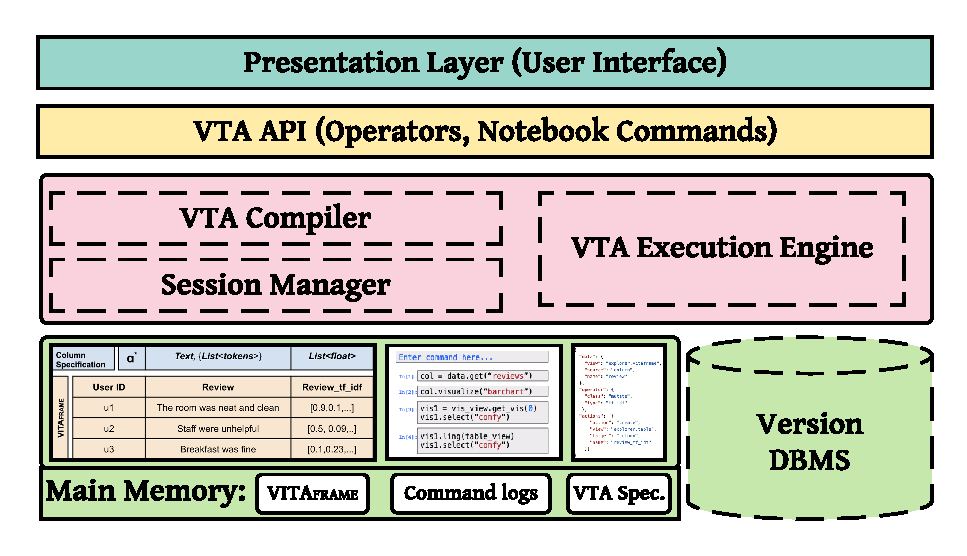
\includegraphics[width=\linewidth]{figures/vita.pdf}
%   \caption{\small \system system architecture.\label{fig:arch}}
%  \vspace{-10pt}
% \end{figure}

% \subsection{Data Model}
% The underlying data structure of \system is a dataframe. \saj{A dataframe is a multi-dimensional array, $A_{mn}$, with a vector of row labels, $R = \{R_1,R_2,\ldots,R_m\}$ and a vector of column labels, $C = \{C_1,C_2,\ldots,C_n\}$~\cite{modin}.} 
% We opted for dataframes instead of databases since 
% \vita tasks
% (\eg training, classification or plotting) cannot always be conveniently performed inside the database~\cite{lajus2014efficient}.
% Dataframes, on the other hand, are widely used in
% exploratory data analysis including \vita due to their coverage of a wide variety of data analysis operators~\cite{modin}. The \emph{Pandas} dataframe API within Python (pandas.pydata.org)
% has been downloaded more than 300 million times and served as a
% dependency for over 265,000 repositories in GitHub. 
% Moreover, dataframes do not require data to
% be defined schema-first allowing flexibility in supported data types and data structures. Finally, dataframes provide a functional interface
% suitable for data science workflows where users can
% progressively compose REPL-style instructions
% to perform ``quick and dirty'' analysis.

% \begin{figure}[!htb] 
% \vspace{-10pt}
%   \centering
%   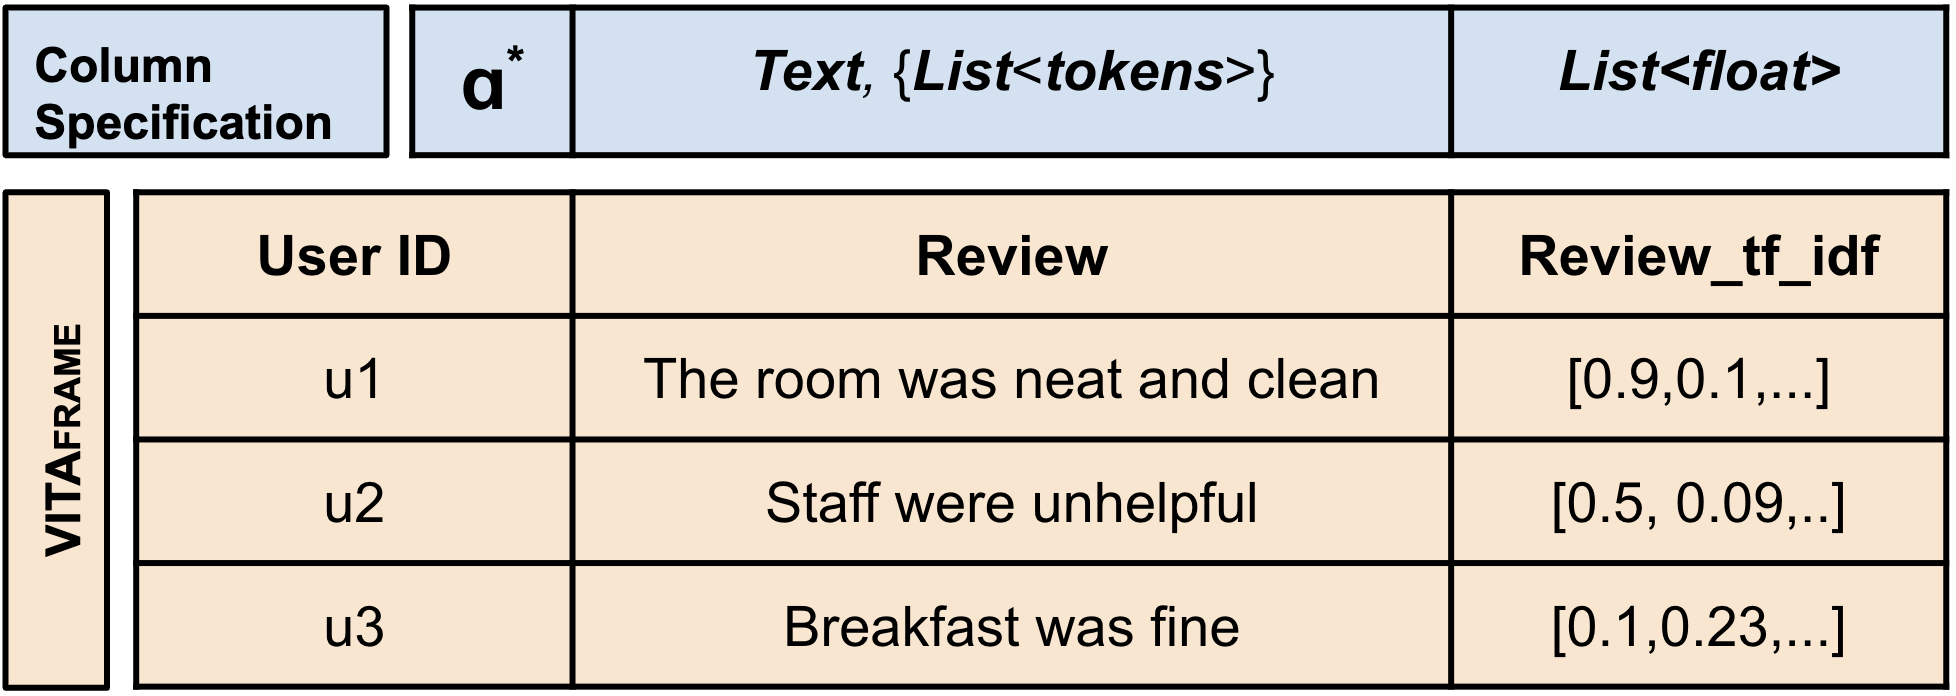
\includegraphics[width=\linewidth]{figures/column_spec.png}
%   \caption{\small \vitaframe data model.\label{fig:column_spec}} 
%   \vspace{-13pt}
% \end{figure}

% To support \vita use-cases we assign a schema to dataframe columns---each column $C_i \in C$ may have a schema defined over a set of data domains, $D = \{d_1, d_2, \ldots\}$ that spans heterogeneous data types like text, visualizations (\textbf{D3}). We call this data structure a \vitaframe. We discuss the underlying data domain for \vita in Section~\ref{sec:vta}.
% As explained in Section~\ref{sec:example}, \vita involves REPL-style workflows where users perform incremental operations on data and examine intermediate results. 
% The intermediate results are also from the data domain, $D$. The intermediate results that have one-to-one correspondence with the a \vitaframe column
% (\eg $n$ reviews are featurized into $n$ feature vectors) is added as a new column. However, these results may not have one-to-one correspondence (\eg dictionary of words in the set of $n$ reviews) and are stored in a separate data structure as a metadata of the corresponding column.
% Therefore, for each column $C_i \in C$ in a \vitaframe, there is a schema specification function $SP_i$ that assigns a domain $d_j \in D$ to the column and a domain $d_k \in D$ for each column metadata.
% For example, in Figure~\ref{fig:column_spec},
% the column \emph{Review\_tf\_idf}'s type is $\mathbf{List}(\mathbf{float})$ and metadata type is $\mathbf{List}(\mathbf{token})$ (\ie the list of unique tokens in the text reviews). Metadata are often used for computing aggregate statistics and visualizations. 
% %For example, to visualize TF-IDF score of top ranked words in the reviews, a user can first construct a new metadata of type $\mathbf{Dictionary}(\mathbf{token}, \mathbf{float})$ that contains the average TF-IDF score of the unique tokens. Then they can use the metadata to create and visualize a ranked list of words as a bar chart (see Figure~\ref{fig:use-case-a}c).
% Note that there can be columns with no metadata.



% \subsection{Computation Model}
% \label{sec:computation}
% \stitle{\vta Compiler.} 
% In Section~\ref{sec:vta}, we present an algebra for specifying \vita workflows, \vta. A user interaction on the front-end are compiled into a \vta specification in \emph{json} format. However, the \vta specifications are incomplete, in the sense that they may omit details ranging from visual encoding such as fonts, line widths to input data type.
% To resolve these ambiguities \system currently 
% uses a rule-based \vta compiler that translates 
% a \vta specification into a detailed specification in lower-level
% operators (see Section~\ref{sec:vta}) for the execution engine to run backend computation. \saj{However, when using Notebook View, users utilize a \vta Python library to issue commands. Again the compiler translates the commands to suitable operators for execution.}  

% \stitle{Execution Engine.} 
% The \vita execution engine takes the following input generated by the \vta compiler: (1) the input data schema in $D$ 
% and (2) the
% user specifications (\eg data transformations, 
% coordinated interactions). 
% The text analysis operations---data preprocessing (\eg cleaning),
% feature extraction (\eg TF-IDF featurization), 
% feature transformation/selection (\eg PCA),
% estimation (\eg classify),
% and more advanced post-processing operations
% (\eg anomaly detection)---are mapped to existing ML and NLP libraries like Spacy, Scikit-learn. While other \vta operators related to visual coordination are mapped to built-in implementations, \eg implementing multi-view coordination (see Section~\ref{sec:vta}).


% \stitle{Version Control.}
% After each operation, \system checkpoints the current state of the \vitaframe as well as the visualizations and notebook commands. However, we haven't yet incorporated a fully functional version control system that may allow fine-grained (\ie at operation level) or coarse-grained (\ie at session level) versioning (\textbf{D5}). We aim to support fine-grained version management of a \vita session involving heterogeneous data types, notebook commands, and user interactions which we discuss in
% Section~\ref{sec:discussion}.


% \subsection{\system Front End}
% \label{sec:ui}
% We have already introduced the four front-end components: Operator View, Table View, Visualization View, and Notebook View, in Section~\ref{sec:intro} (see Figure~\ref{fig:fe}). These components satisfy our first design consideration of having an integrated environment for in-place text analytics (\textbf{D1}).

% Using Operator View (see Figure~\ref{fig:fe}a) users can perform various \vita operations on the other views. For example, cleaning the data in Table View, adding visual summaries in Visualization View. The operations are mapped to \vta specifications.
% Table View (see Figure~\ref{fig:fe}b) is inspired by traditional spreadsheets and tabular data visualization tools~\cite{spenke1996focus} and enables users to directly operate on the data, a feature missing from notebooks and visualization tools. 
% Table View data can be transformed into visual summaries like barcharts and scatterplots using the visualizations operators either in Operator View or Notebook View (see Figure~\ref{fig:fe}). Moreover, a cell in Table View can also be a visualization, similar to tabular data analytics tools~\cite{spenke1996focus}. 
% The visualizations in Visualization View (see Figure~\ref{fig:fe}c) are displayed as a carousel of charts. To create interactive visualizations, we use \emph{Vega-Lite}~\cite{satyanarayan2016vega}  for visual encoding and the \emph{Vega} signals~\cite{satyanarayan2015reactive} for interaction specification.
% Notebook View design (see Figure~\ref{fig:fe}d) is inspired by computational notebooks and enables users to perform \vita operation using the Python-based \vta library.  All of the views in \system can coordinate with each other---interactions on one view are reflected in other views (\textbf{D2}). Through \vta, users can declaratively specify interactive coordination (\eg brush-and-linking) between these views (\textbf{D2}). In the next section, we discuss how users can specify such coordination. 

%\stitle{View Coordination.}
%We explain in Section~\ref{sec:vta}, how \vta enhances the Vega-lite interaction grammar to enable  coordination between  views.Through \vta, users can declaratively specify interactive coordination (\eg brush-and-linking) between visualizations in Visualization View. For example, as shown in Figure~\ref{fig:use-case-b}, clicking on a bar (word) in  the bar chart visualization of top-words can highlight the points in a scatterplot, where each point corresponds to a review, indicating these reviews contain that word. Users' interaction on other views may also be coordinated with visualizations in the Visualization View. For example, selecting a review in Table View may highlight both the relevant top-word in the bar chart and multiple points in the scatterplot.



% \section{\system: In-situ Analysis}
% \label{sec:system}
% \sajreview{In this section, we discuss the current progress in developing \system. We first explain the system architecture for enabling \vita with the tool and then present the user interface components. Figure~\ref{fig:arch} shows the overview of the \system system architecture. The components with dashed borders (``- -'') are partially implemented and require further refinement.}


% \begin{figure}[!htb] 
% \vspace{-10pt}
%   \centering
%   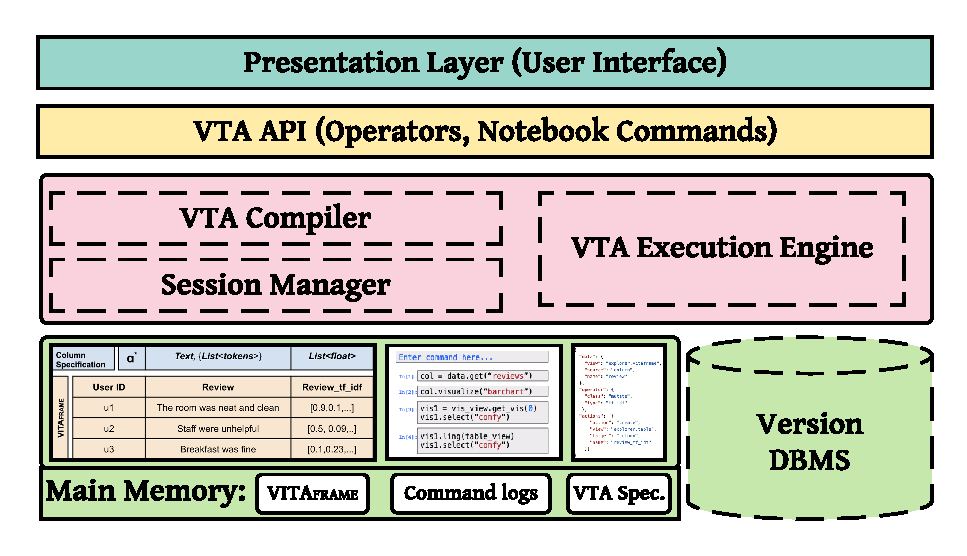
\includegraphics[width=\linewidth]{figures/vita.pdf}
%   \caption{\small \system system architecture.\label{fig:arch}}
% \end{figure}

% \subsection{Data Model}
% \sajreview{The underlying data structure of \system is a dataframe. 
% We opted for dataframes instead of databases since 
% \vita tasks
% (\eg training, classification or plotting) cannot always be conveniently performed inside the database~\cite{lajus2014efficient}.
% Dataframes, on the other hand, are widely used in
% exploratory data analysis including \vita; for example,
% the \emph{pandas} dataframe API within Python (pandas.pydata.org)
% has been downloaded more than 300 million times and served as a
% dependency for over 265,000 repositories in GitHub. 
% Besides their ubiquity, dataframes are incredibly popular in \vita 
% due to their coverage a wide variety of data analysis operators
% like relational (\eg \emph{filter, join}) and linear algebraic \emph{transpose})
% operations. Moreover, dataframes do not require data to
% be defined schema-first allowing flexibility in supported data types and data structures. Finally, dataframes provide a functional interface
% suitable for data science workflows where users can
% progressively compose REPL-style instructions
% to perform ``quick and dirty'' analytics.
% To support \vita use-cases we extend existing formalization of dataframes~\cite{modin,lara}---a dataframe in \system is a multi-dimensional array with a vector of row labels and a vector of column labels where each column may have a schema defined over a set of data domains, $D = \{d_1, d_2, \ldots\}$ that spans heterogeneous data types like text, visualizations (\textbf{D3}). The underlying data domain for \vita is explained in Section~\ref{sec:vta}.}

% \begin{figure}[!htb] 
% \vspace{-10pt}
%   \centering
%   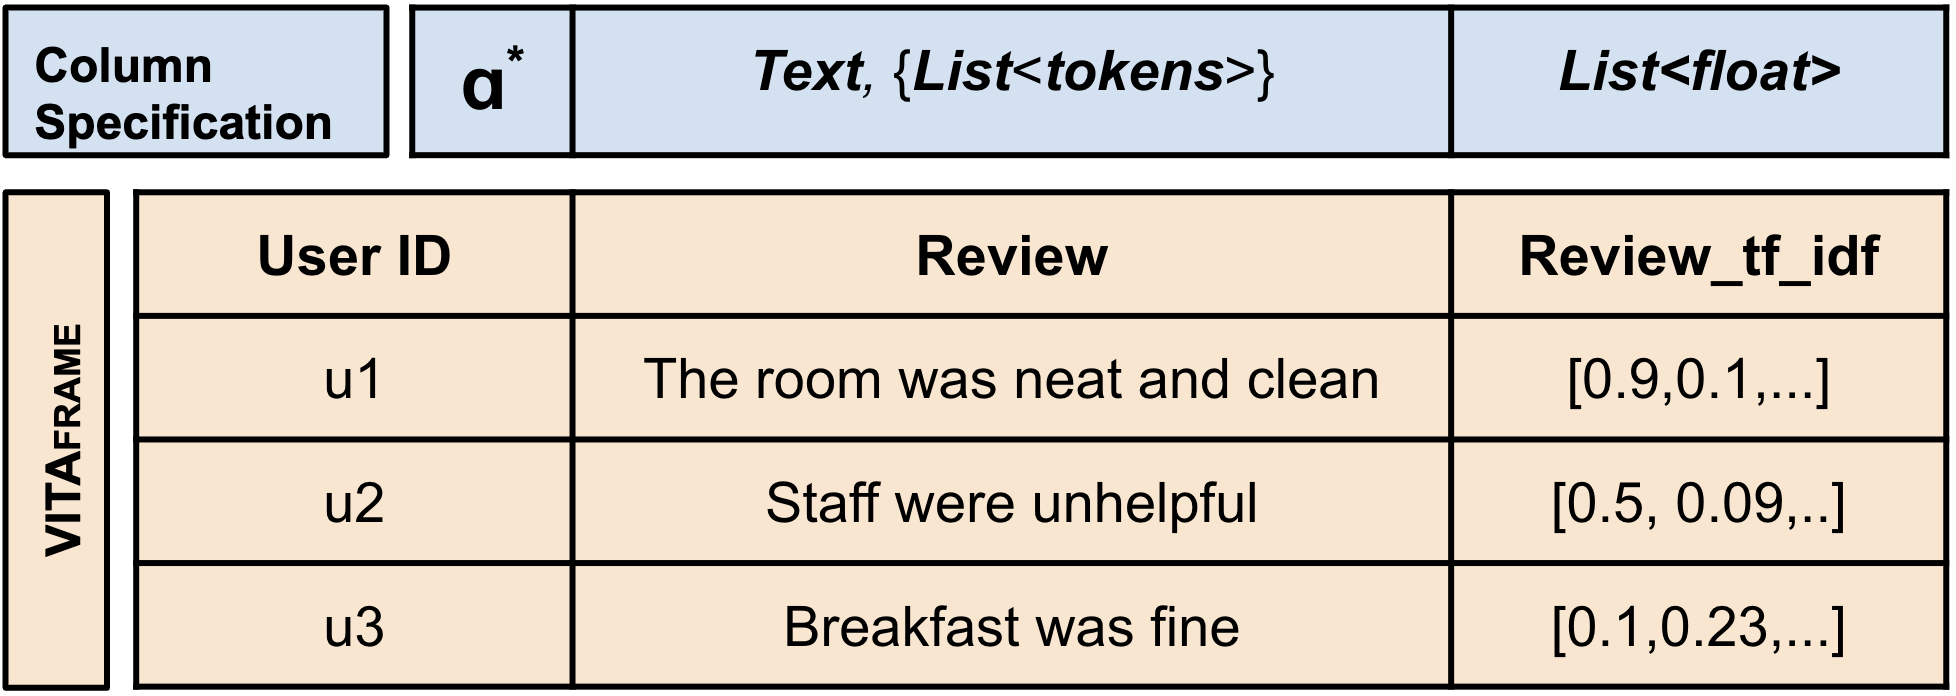
\includegraphics[width=\linewidth]{figures/column_spec.png}
%   \caption{\small \vitaframe data model.\label{fig:column_spec}} 
%   \vspace{-15pt}
% \end{figure}
% %\stitle{Column Specification.} 
% As explained earlier, \vita involves REPL-style workflows where users perform incremental operations on data and examine intermediate results. \hide{For example, in the use-case explained earlier, the user first cleans the data, then featurizes the cleaned data, and then finally performs a number of analytical operations, each time validating the intermediate results.}
% The intermediate results are also from the data domain, $D$. These intermediate results are either mapped or metadata. Mapped data have one-to-one correspondence with the \vitaframe column
% (\eg $n$ reviews are featurized into $n$ feature vectors) and are added as a new column. Metadata may not have one-to-one correspondence (\eg dictionary of words in the set of $n$ reviews) and are stored in separate data structure.
% Therefore, for each column $C_i$ in a \vitaframe there is a \emph{specification} function $SP_i$ that assigns a domain $d_i \in D$ to the column and a domain $d_{ij} \in D$ for each metadata $j$.
% For example, in Figure~\ref{fig:column_spec},
% the column \emph{review\_tf\_idf}'s type is $\mathbf{List}(\mathbf{float})$ and metadata type is $\mathbf{List}(\mathbf{token})$ (\ie the list of unique tokens in the text reviews). Metadata are often used for computing aggregate statistics and visualizations. For example, to visualize TF-IDF score of top ranked words in the reviews, a user can first construct a new metadata of type $\mathbf{Dictionary}(\mathbf{token}, \mathbf{float})$ that contains the average TF-IDF score of the unique tokens. Then they can use the metadata to create and visualize a ranked list of words as a bar chart.
% Note that there can be columns with no metadata.


% \system currently supports persistence of only the latest session data.
% After each operation that performs data updates, we checkpoint the \vitaframe by storing the new version as a serialized file. However, we don't  maintain a version graph in the current implementation. Our ultimate goal is to support more fine-grained version management of heterogeneous data types, notebook commands, and user interactions which we discuss in
% Section~\ref{sec:discussion} (\textbf{D5}).


% \begin{figure*}[!htb]
% \centering
% \begin{tabular}{ c c c}
%   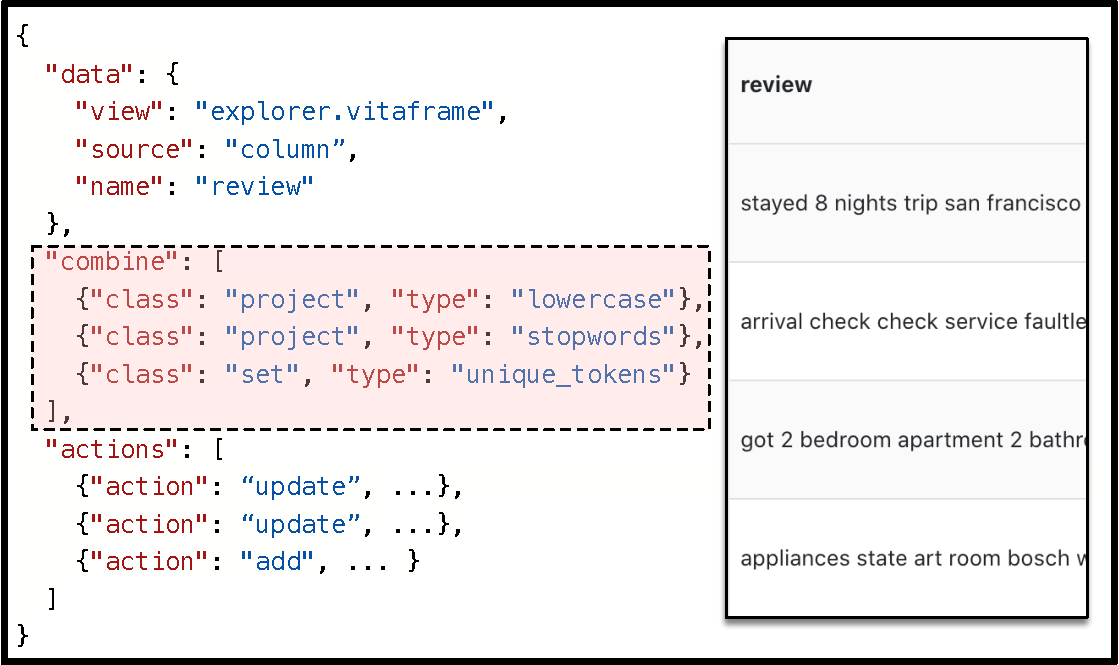
\includegraphics[width=0.3\linewidth,height=0.18\linewidth]{figures/combine_clean.pdf}   & 
%   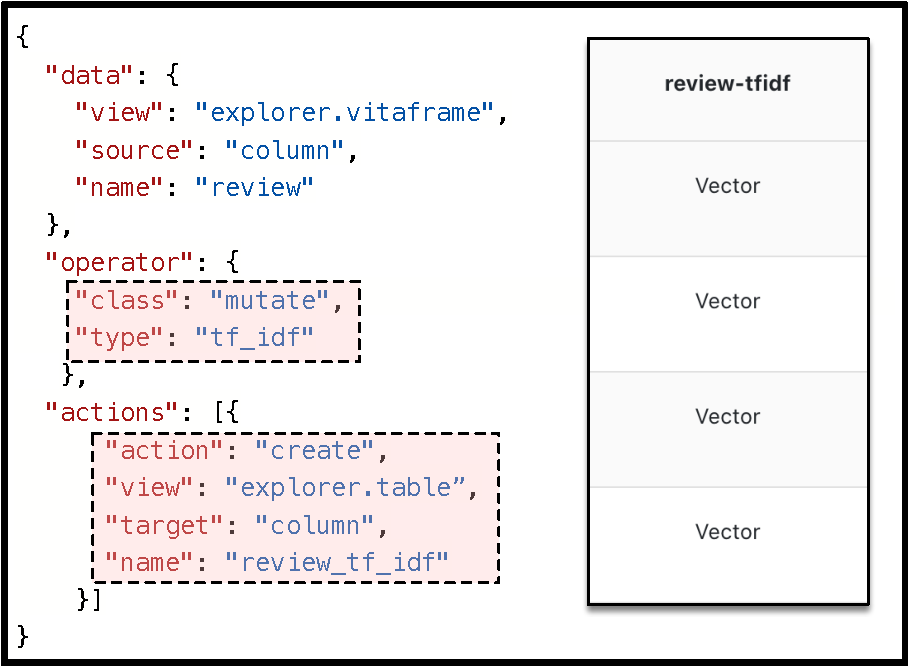
\includegraphics[width=0.3\linewidth,height=0.18\linewidth]{figures/tf_idf.pdf} & 
%   \includegraphics[width=0.4\linewidth,height=0.18\linewidth]{figures/bar chart.pdf} \\
%      (a) Clean and generate metadata & 
%      (b) Create TF-IDF feature vector &
%      (c) Visualize top-words by TF-IDF score
% \end{tabular}
%     \caption{\small Example of \vta specification. (a) Use \emph{Combine} operator to clean data (\eg \emph{lowercasing}, \emph{stopwords removal}) and generate metadata (\eg \emph{unique\_token} to create token dicitionary) for use in subsequent steps. (b) Define featurization operation and subsequent action, \ie column creation in Table View. (c) Compute average TF-IDF score of each token in the dictionary using \emph{aggregate} operator and then create bar chart of top-ranked words using \emph{visualize} operator.}
% \vspace{-15pt}
%     \label{fig:use-case-a}
% \end{figure*}

% \subsection{Computation Model}
% \label{sec:computation}
% \stitle{\vta Compiler.} 
% \sajreview{In Section~\ref{sec:vta}, we present a grammar for specifying \vita workflows, \vta, that spans
% text preprocessing, featurization,
% visualization, post-processing, coordinated interactions 
% (\textbf{D4}). Like other highlevel grammars, the \vta specifications are incomplete, in the sense that
% they may omit details ranging from
% visual encoding such as fonts, line widths to input data type.
% The current \vta compiler is rule-based, \ie uses a rule-based system to resolve these ambiguities and translates 
% \vta specification into a detailed specification in lower-level
% operators (see Section~\ref{sec:vta}) for the execution engine to run backend computation.}


% \stitle{Execution Engine.} 
% The \vita execution engine takes the following input generated by the \vta compiler: (1) the input data schema in $D$ 
% and (2) the
% user specifications (\eg data transformations, analysis operations
% coordinated interactions). 
% The text analysis operations, \ie data preprocessing (\eg cleaning),
% feature extraction (\eg TF-IDF featurization), 
% feature transformation/selection (\eg PCA),
% estimation (\eg classify),
% and more advanced post-processing operations
% (\eg anomaly detection), are mapped to existing ML and NLP libraries like Spacy, Scikit-learn. While other \vta operators related to visual coordination are mapped to built-in specifications.


% \stitle{Version Control.}
% \sajreview{
% As mentioned earlier, \system currently supports checkpointing upto the most recent operation of a \vita session. A naive approach to persisting the \vita sessions is to assign a unique version identifier to serialized \vitaframe, notebook command logs, and visualizations. However, we aim to support fine-grained session persistance and version control for various components. We outline the vision for version control system for \vita workflows in Section~\ref{sec:discussion}.
% }

% \subsection{\system Front End}
% \label{sec:ui}
% \sajreview{In this section, we present the user interface of \system and explain the scope of operations supported.
% We have already introduced the four front-end components, \ie Operator View, Table View, Visualization View, and Notebook View, in Section~\ref{sec:intro} (see Figure~\ref{fig:fe}). These components satisfy our first design consideration of having an integrated environment for in-place text analytics (\textbf{D1}). Moreover, the user interface is essentially a multiple coordinated view where interactions on one view maybe reflected on other view(s) (\textbf{D2}). We discuss the components and the supported interactions next.}



% \stitle{Operator View.}
% \sajreview{Using Operator View (see Figure~\ref{fig:fe}a) users can perform various operations on the other views. For example, \emph{cleaning} the data in Table View, adding \emph{visual summaries} in Visualization View. All of the operators in this view are designed based on the visual text algebra (see Section~\ref{sec:vta}). The operators are mapped to \vta specifications that are sent to the backend for execution.
% While the interactions on Operator View impacts both the table and Visualization View, the coordination is not bidirectional---interaction on these views never impact Operator View.}

% \stitle{Table View.}
% \sajreview{Table View (see Figure~\ref{fig:fe}b) is inspired by traditional spreadsheets and tabular data visualization tools. Table View provides a direct manipulation interface for users to directly operate on the data, a feature missing from notebooks and visualization tools. Some operators in Operator View add new columns to Table View. %For example, in our use-case, performing TF-IDF featurization adds a column corresponding to each review in the dataset.
% Table View data can be transformed into visual summaries like barcharts and scatterplots using the \emph{visualization} operator in Operator View (see Figure 1). Moreover, a cell in Table View can also be a visualization, similar to tabular data analytics tools~\cite{spenke1996focus}. Users can interact with visualizations in the Visualization View to impact Table View presentation and vice-versa (summary-table coordination), which we discuss next.}


% \stitle{Summary View.}
% \sajreview{The visualizations in Visualization View (see Figure~\ref{fig:fe}c) are displayed as a carousel of charts. We create the visualizations using \emph{Vega-Lite}~\cite{satyanarayan2016vega} and enable rich set of interactions on the visualizations by using \emph{Vega} signals API~\cite{satyanarayan2015reactive}. We explain in Section~\ref{sec:vta}, how \vta enhances the \emph{Vega-lite} interaction grammar to enable  coordination with other views. A visualization can coordinate with other visualizations in the Visualization View as well as other views in \system. For example, as shown in Figure~\ref{fig:use-case-b}, clicking on a bar (word) in the bar chart visualization of top-words can highlight the points in a scatterplot, where each point corresponds to a review, indicating these reviews contain that word. Users interaction on other views may also be coordinated with visualizations in the Visualization View. For example, selecting a review in Table View may highlight both the relevant top-word in the bar chart and multiple points in the scatterplot.}

% \stitle{Notebook View.}
% \sajreview{Notebook View design (see Figure~\ref{fig:fe}d) is inspired by computational notebooks and enables users to perform \vita operation using the a python-based \vta library.  Users can even interact with visualizations in the Visualization View or columns in Table View by writing commands in Notebook View. For example, user can select a bar (\eg the word ``comfy'') in the bar chart shown in Figure~\ref{fig:use-case-a}c via the following \vta command:}
% \vspace{-4pt}
% \begingroup\makeatletter\def\f@size{8}\check@mathfonts
% %\color{blue}
% \begin{align*}
% ln[1]: \quad & \tt     bar chart \ \ = \ \ summary\_view.get\_vis(0)\\
%             & \tt     bar chart.select(``comfy'') 
% \end{align*}
% %\vspace{-10pt}
% \endgroup


